% Update 5 Sep 2018-YC
% Update 6 Sep 2018-YC
% Update 11 Sep 2018-SR
% Update 11 Sep 2018-YC
% Update 12 Sep 2018-YC

\documentclass[12pt,onecolumn]{IEEEtran}
%\documentclass[journal,twoside]{IEEEtran}
\usepackage{cite}
\usepackage[table]{xcolor}
\usepackage{xcolor}
%\usepackage{filecontents}
%\usepackage{titling}
%\usepackage{fullpage} % Package to use full page
%\usepackage{parskip} % Package to tweak paragraph skipping

\usepackage{tikz} % Package for drawing
\usetikzlibrary{arrows}

\usepackage{amsmath}
\usepackage{amsthm}
%\usepackage{hyperref}
%\usepackage{apacite}
\usepackage{amssymb, url}
\usepackage[long]{optidef}
\usepackage{multirow}
\usepackage{graphicx,booktabs}
%\usepackage[style=ieee]{biblatex}


%\usepackage{fixltx2e}
%\usepackage{stfloats}
\usepackage{dblfloatfix}


\theoremstyle{plain}
\newtheorem{proposition}{Proposition}
\theoremstyle{definition}
\newtheorem{definition}{Definition}


\begin{document}

\title{Capacity Market Formulation}
\date{}

%\author{Sepehr~Ramyar,~\IEEEmembership{Student Member,~IEEE,}
%        and~Yihsu~Chen,~\IEEEmembership{Member,~IEEE}% <-this % stops a space
%\IEEEcompsocitemizethanks{\IEEEcompsocthanksitem Electrical and Computer Engineering, Jack Baskin School of Engineering, University of California Santa Cruz, Santa Cruz,
%CA, 95064.\protect\\
%% note need leading \protect in front of \\ to get a newline within \thanks as
%% \\ is fragile and will error, could use \hfil\break instead.
%E-mail: yihsuchen@ucsc.edu}
%%\IEEEcompsocthanksitem J. Doe and J. Doe are with Anonymous University.}% <-this % stops an unwanted space
%\thanks{}}
%
%
%\markboth{IEEE Transactions on Power Systems}{A Power Market Model In Presence of Strategic Prosumers}

\maketitle

\subsection{Notations}
We use capital letters to indicate parameters and sets. 
Lowercase letters refer to variables and indices. 
Dual variables are designated with greek lower-case letters. 
In the following presentation, ``$x \perp y$'' implies $x^Ty=0$.)

1) Sets and Indices
\begin{IEEEdescription}[\IEEEusemathlabelsep\IEEEsetlabelwidth{$V_1,V_2,V_3$}]
\item[$f \in F$] Set of generation firms.
\item[$i \in I$] Set of nodes in the network.
\item[$h \in H$] Set of generation units.
\item[$H_{fi} \in H$] Set of generating units at node $i$ owned by firm $f$'s .
\item[$k \in K$] Set of transmission branchs, lines or flowgates.
\item[$t \in T$] Set of seasons including peak and off-peak. $T = \{\text{\textit{peak, off-peak}}\}$
\end{IEEEdescription}

2) Parameters
\begin{IEEEdescription}[\IEEEusemathlabelsep\IEEEsetlabelwidth{$V_1,V_2,V_3$}]
\item[$PTDF_{ki}$] Power transmission distribution factor for a unit of power. injected at hub and withdrawn at node $i$ through branch $k$.
\item[$P_{it}^0$] Vertical intercept of the inverse demand function for node $i$ (\$/MWh).
\item[$Q_{it}^0$] Horizontal intercept of the inverse demand function for node $i$ (MW).
\item[$T_k$] Upper bound of thermal limit for branch $k$ (MW).
\item[$X_{fih}$] Production capacity for generation unit $h$ belonging to firm $f$ at node $i$.
\item[$K_i$] Exogenous renewable output possessed by the prosumer at node $i$ (MW).
\item[$G_i$] Production capacity of the prosumer's dispatchable unit at node $i$ (MW).
\item[$A^0_i$] Vertical intercept of the inverse function representing prosumer's marginal benefit for consumption at node $i$ (\$/MWh).
\item[$B^0_i$] Horizontal intercept of the inverse function representing prosumer's marginal benefit for consumption at node $i$ (MW).
\end{IEEEdescription}

3) Primal Variables
\begin{IEEEdescription}[\IEEEusemathlabelsep\IEEEsetlabelwidth{$V_1,V_2,V_3$}]
\item[$p_{it}$] Wholesale power price at node $i$ in season $t$ (\$/MW).
\item[$z_{fit}$] Sales by prosumer at node $i$ to firm $f$ in season $t$ (MW)
\item[$b_{fit}$] Purchase by prosumer at node $i$ from firm $f$ in season $t$ (MW)
\item[$l_{it}$] Prosumer's demand at node $i$ in season $t$ (MW)
\item[$g_{it}$] Power provided by prosumer's dispatchable (or backup) resource at node $i$ in season $t$ (MW)
\item[$x_{fiht}$] Power generated by unit $h$ owned by firm $f$ at node $i$ in wholesale market in season $t$ (MW).
\item[$s_{fit}$] Sales by firm $f$ at node $i$ in season $t$ (MW).
\item[$w_{it}$] Transmission price charged by grid owner to move power from hub to node $i$ in season $t$ (\$/MW).
\item[$a_{it}$] Amount of power sell (+) or buy )-) by arbitrager at node $i$ in season $t$ (MW).
\item[$d_{it}$] Wholesale demand from the consumer pool at node $i$ in season $t$ (MW).
\item[$y_{it}$] Amount of power injected (+) to or withdrew from (-) hub to node $i$ in season $t$ (MW)
\item[$B_t$] Number of hours in each period; 8000 for off-peak and 760 for peak period
\end{IEEEdescription}

4) Dual Variables
\begin{IEEEdescription}[\IEEEusemathlabelsep\IEEEsetlabelwidth{$V_1,V_2,V_3$}]
\item[$\lambda_{kt}$] variable of to branch $k$ limits in season $t$ (\$/MW).
\item[$\rho_{fiht}$] Dual variable of capacity constraint of unit $h$ of firm $f$ at node $i$ in season $t$ in season $t$ (\$/MW).
\item[$\theta_{ft}$] Dual variable of firm $f$'s supply and demand balance condition in season $t$ (\$/MW).
\item[$\delta_{it}$] Dual variable of prosumer's power balance constraint in season $t$ (\$/MW).
\item[$\kappa_{it}$] Dual variable of prosumer's dispatchable generation capacity in season $t$ (\$/MW).
\item[$\mu_{it}$] Dual variable of prosumer's sales limit constraint in season $t$ (\$/MW).
\end{IEEEdescription}

5) Capacity Investment Variables and Parameters
\begin{IEEEdescription}[\IEEEusemathlabelsep\IEEEsetlabelwidth{$V_1,V_2,V_3$}]
\item[$x^{new}_{fiht}$] Power generated by \textit{future} unit $h$ owned by firm $f$ at node $i$ in wholesale market in season $t$(MW).
\item[$x^{cap}_{fih}$] Production capacity for generation \textit{future} unit $h$ belonging to firm $f$ at node $i$.
\item[$\rho^{new}_{fiht}$] Dual variable of \textit{new} capacity constraint of unit $h$ of firm $f$ at node $i$ in season $t$ (\$/MW).
\item[$INV_{fih}$] Annualized capacity cost $\frac{\frac{\$}{MW}}{year}$.
\item[$D_{it}$] Demand margin for node $i$ in season $t$.
\end{IEEEdescription}

\section{Agent Problem Formulations}
In this section, each agent's optimization problem is formulated.

\subsection{Generators}
A supplier $f$'s problem is given as follows:
\begin{maxi!}[3]
	{s_{fit},x_{fiht}}{\sum_{i,f,t}B_t(p_{it}-w_{it})(s_{fit}-z_{fit})} {\label{e2}}{} \breakObjective{- \sum_{fiht}B_t\left(C_{fih}(x_{fiht}) - w_{it} x_{fiht}\right) \nonumber}
	\breakObjective{-\sum_{fiht}B_t\left(C_{fiht}(x^{new}_{fiht}) - w_{it} x^{new}_{fiht})
	+ x^{cap}_{fih} INV_{fih}\right) \nonumber}
\addConstraint{x_{fiht}}{\leq X_{fih}}{\qquad(\rho_{fiht})}{\label{2b}}
\addConstraint{x^{new}_{fiht}}{\leq x^{cap}_{fih}}{\qquad(\rho^{new}_{fiht})}{\label{2b}}
\addConstraint{\sum_{i} s_{fit} - z_{fit} - \sum_{ih}x_{fiht} - \sum_{ih}x^{new}_{fiht} }{= 0}{\qquad(\theta_{ft})}{\label{2c}}
	\addConstraint{s_{fit}, x_{fiht},x^{new}_{fiht},x^{cap}_{fih} \geq 0} \nonumber
\end{maxi!}

\subsection{Consumers}
Consumers maximize their benefit that is utility of consumption minus payment for power:
\begin{align}
\max_{d_{ti}>D_{ti}} \sum_t B_t [P^0_{ti}D_{ti} + \int^{d_{ti}}_{D_{ti}}P(x)dx - p_{ti}d_{ti}], \qquad \forall i,t \label{demand}
\end{align}
where $t$ indicates the \textit{peak} or \textit{off-peak} period of the year (i.e., $t \in \{\text{\textit{peak, off-peak}}\}$) and $P^0_{ti}$ and $Q^0_{ti}$ represent the \textit{price cap} and max consumption for the corresponding season, respectively. This is shown in Fig.\ref{price_cap}.

\begin{figure}
\centering
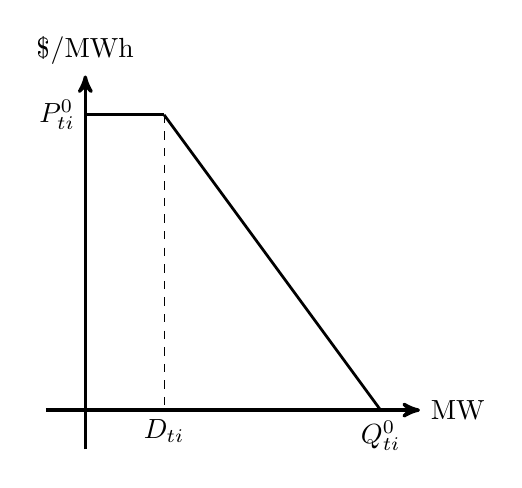
\begin{tikzpicture}[
    scale=5,
    axis/.style={very thick, ->, >=stealth'},
    important line/.style={thick},
    dashed line/.style={dashed, thin},
    pile/.style={thick, ->, >=stealth', shorten <=2pt, shorten
    >=2pt},
    every node/.style={color=black}
    ]
\draw[axis] (-0.1,0)  -- (0.85,0) node(xline)[right]{$\text{MW}$};
\draw[axis] (0,-0.1) -- (0,0.85) node(yline)[above] {\$/$\text{MWh}$};
\draw[line width=0.35mm, black](0,0.75)node[left]{$P^0_{ti}$}--(0.2,0.75) ;
\draw[line width=0.35mm, black](0.2,0.75)--(0.75,0)node[below]{$Q^0_{ti}$};;
\draw[dashed](0.2,0.75)--(0.2,0)node[below]{$D_{ti}$};
\end{tikzpicture}
\caption{An illustration of demand function with price cap}
\label{price_cap}
\end{figure}


\subsection{Prosumer}
Prosumer's optimization problem is as follows:

\begin{maxi!}[3]
	{z_{fit},l_{it},g_{it}}{\sum_t B_t [ p_{it} \sum_f z_{fit} - {\int^{K_{ti}}_{l_i} B'_{ti}(x)dx}- C^g_i(g_{it})]\protect\label{1a}}{\label{e1}}{}
	\addConstraint{\sum_fz_{fi} + l_{it} - K_{ti} - g_{it}}{\leq 0}{\qquad(\delta_{it})}{\label{1b}}
	\addConstraint{g_{it}}{\leq G_i}{\qquad(\kappa_{it})}{\label{1c}}
	\addConstraint{-\sum_f z_{fi} - l_{it}}{\leq 0}{\qquad(\mu_{it})}{\label{1d}}
	%\addConstraint{z_{fi},b_{fi},l_i,g_i}{\geq 0}.{\label{1e}}\nonumber
\end{maxi!}

\subsection{Grid Owner}
The grid owner operates the power network and decides on the allocation of transmission resources while charging producers $w_{it}$ to move power from hub to node $i$ in season $t$. The optimization problem faced by the grid operator is given in (\ref{e5}). 
\begin{maxi!}[3]
	{y_{it}}{\sum_{i,t}B_t w_{it} y_{it} \protect\label{5a}}{\label{e5}}{}
	\addConstraint{-T_k}{\leq \sum_i PTDF_{ki} y_{it}}{\leq T_k}{\qquad(\lambda_{kt})}{\label{5b}}
\end{maxi!}


\section{Optimality and Market Clearing Conditions}

\subsection{Generators' FOCs}
\begin{subequations}\label{eq:KKT_Supply}
\begin{align}
&0 \leq s_{fit} \perp  B_t(p_{it} - w_{it}) -\theta_{ft} \leq 0, \qquad  \forall i,t  \\
&0 \leq x_{fiht} \perp B_t(-C'(x_{fiht}) + w_{it}) - \rho_{fiht} + \theta_{ft} \leq 0, \qquad \forall i,t, h \in H_{fi}  \\
&0 \leq x^{new}_{fiht} \perp B_t(- C'(x^{new}_{fiht}) + w_{it}) - \rho^{new}_{fiht} + \theta_{ft} \leq 0, \qquad \forall i,t, h \in H_{fi}  \\
& 0 \leq x^{cap}_{fih} \perp -INV_{fih} + \rho^{new}_{fiht} \leq 0, \qquad \forall f,i,t, h \in H_{fi}\\
& \sum_{i} s_{fit} - z_{fit} - \sum_{ih}x_{fiht} - \sum_{ih}x^{new}_{fiht} = 0, \qquad  \forall f,t \\
&0 \leq \rho_{fiht} \perp x_{fiht}-X_{fih} \leq 0, \qquad  \forall i,t, h \in H_{fi}\\
&0 \leq \rho^{new}_{fih} \perp x^{new}_{fiht}-x^{cap}_{fih} \leq 0, \qquad  \forall i,t, h \in H_{fi}
\end{align}
\end{subequations}


\subsection{Prosumer FOCs}

\begin{subequations}
\label{e8}
\begin{align}
& B_t p_{it} - \delta_{it} = 0, \qquad \forall f,i,t	\label{8a}\\
%& \text{For } z_{fi}: p_i - (P^0_i/Q^0_i)\sum_fz_{fi} - \delta_i = 0,\forall f,i\tag{3a*} \label{8e} \\
& 0 \leq l_{it} \perp B_t(A^0_{it} - B^0_{it} l_{it}) - \delta_{it}  \leq 0, \qquad \forall i,t  \label{8b}  \\
& 0 \leq g_{it}  \perp - B_t C^{g\prime}_i(g_{it}) -\kappa_{it} + \delta_{it}  \leq 0, \qquad \forall i,t \label{8c}\\
& l_{it} - K_{it} - g_{it} + \sum_f z_{fit}= 0, \qquad \forall i,t \\
& 0 \leq \kappa_i  \perp  g_{it} - G_i \leq 0, \qquad \forall i,t \label{8d}
\end{align}
\end{subequations}

\subsection{Grid Owner FOCs}
\begin{subequations}\label{e10}
\begin{align}
& B_t w_{it} - \sum_{k} PTDF_{ki}(\lambda_{kt}^+ - \lambda_{kt}^-) = 0 & \forall i,t \\
&0 \leq \lambda_{kt}^+ \perp \sum_i PTDF_{ki}y_{it} - T_{k} \leq 0 &  \forall k,t \\
&0 \leq \lambda_{kt}^- \perp -\sum_i PTDF_{ki}y_{it} - T_{k} \leq 0 & \forall k,t
\end{align}
\end{subequations}


\subsection{Consumer FOCs}
\begin{align}
0 \leq d_{it} \perp p_{it} -\big(P^0_{it} - ({P^0_{it}}/{Q^0_{it}})d_{it}\big) \geq 0 , \qquad \forall i = 1, \ldots, I, t \in \{\text{\textit{peak,off-peak}}\} \label{demand}
\end{align}

\end{document}